%-------------------Packages----------------------
\documentclass[12pt,letterpaper, USenglish]{article}
\usepackage[latin1]{inputenc}
\usepackage[table, dvipsnames]{xcolor}
\usepackage{amsmath}
\usepackage{amsfonts}
\usepackage{amssymb}
\usepackage{amsthm}
\usepackage{graphicx}
\usepackage{mathtools}
\usepackage{verbatim}
\usepackage{hyperref}
\usepackage{array}
\usepackage{float}
\usepackage{tikz}
\usepackage{thmtools}
% \usepackage{todonotes}
\usepackage{indentfirst}
\usepackage{thm-restate}
\usepackage[left=1.00in, right=1.00in, top=1.00in, bottom=1.00in]{geometry}
\usepackage{isodate}
\usepackage[ruled,vlined]{algorithm2e}

\graphicspath{{./}}
\tolerance=1
\emergencystretch=\maxdimen
\hyphenpenalty=10000
\hbadness=10000

%---------------Declare commands------------------
\DeclarePairedDelimiter\ceil{\lceil}{\rceil}
\DeclarePairedDelimiter\floor{\lfloor}{\rfloor}
\renewcommand\qedsymbol{$\blacksquare$}
\renewcommand{\listtheoremname}{List of Theorems}
\tikzstyle{line} = [draw, thick, color=black]

%--------------Define colors----------------------
\definecolor{bubbles}{rgb}{0.91, 1.0, 1.0}
\definecolor{columbiablue}{rgb}{0.61, 0.87, 1.0}
\definecolor{lightcyan}{rgb}{0.88, 1.0, 1.0}

%--------------Define numbering-------------------
\newtheorem{theorem}{Theorem}
\newtheorem{lemma}{Lemma}
\newtheorem{corollary}{Corollary}
\theoremstyle{definition}
\newtheorem*{definition*}{Definition}
\declaretheorem[name=Definition]{definition}
\newtheorem{example}{Example}

\pagenumbering{gobble}

\numberwithin{theorem}{section}
\numberwithin{lemma}{section}
\numberwithin{corollary}{section}
\numberwithin{definition}{section}
\numberwithin{example}{section}
\numberwithin{equation}{theorem}

%---------------Title info------------------------

\title{Tensile Testing Assistant User Manual}
\author{Kaitlin Dosch \and Chris Geidans \and Connor May \and Julia VanLandingham}
\date{\today}

\begin{document}
%-----------------Title---------------------------
\maketitle

\pagebreak
%------------Table of Contents--------------------
\tableofcontents
\pagebreak
\pagenumbering{arabic}

%----------todo list for editing------------------
\pagebreak

\section{Product Purpose}\label{purposeSection}
The purpose of this application is to assist in testing the tensile strength of materials.
This software is designed to pull force and elongation data from the appropriate machines through a connected National Instruments device. This data allows for the stress-strain graph to be drawn in real time using the corresponding cross-section and gauge length values input by the user. Lastly, the data can be exported to a CSV file that can then be opened and manipulated in Excel easily. 

\section{Operation Guide}\label{operationSection}
Upon start up, the user will see a screen depicting an empty graph with buttons labeled ``Input,'' ``Start,'' ``Clear,'' and ``Export'' along the bottom. Options for measurement input, settings configuration, and data exporting are also accessible in appropriate menus along the top of the screen. 

\begin{figure}[H]
    \centering
    \frame{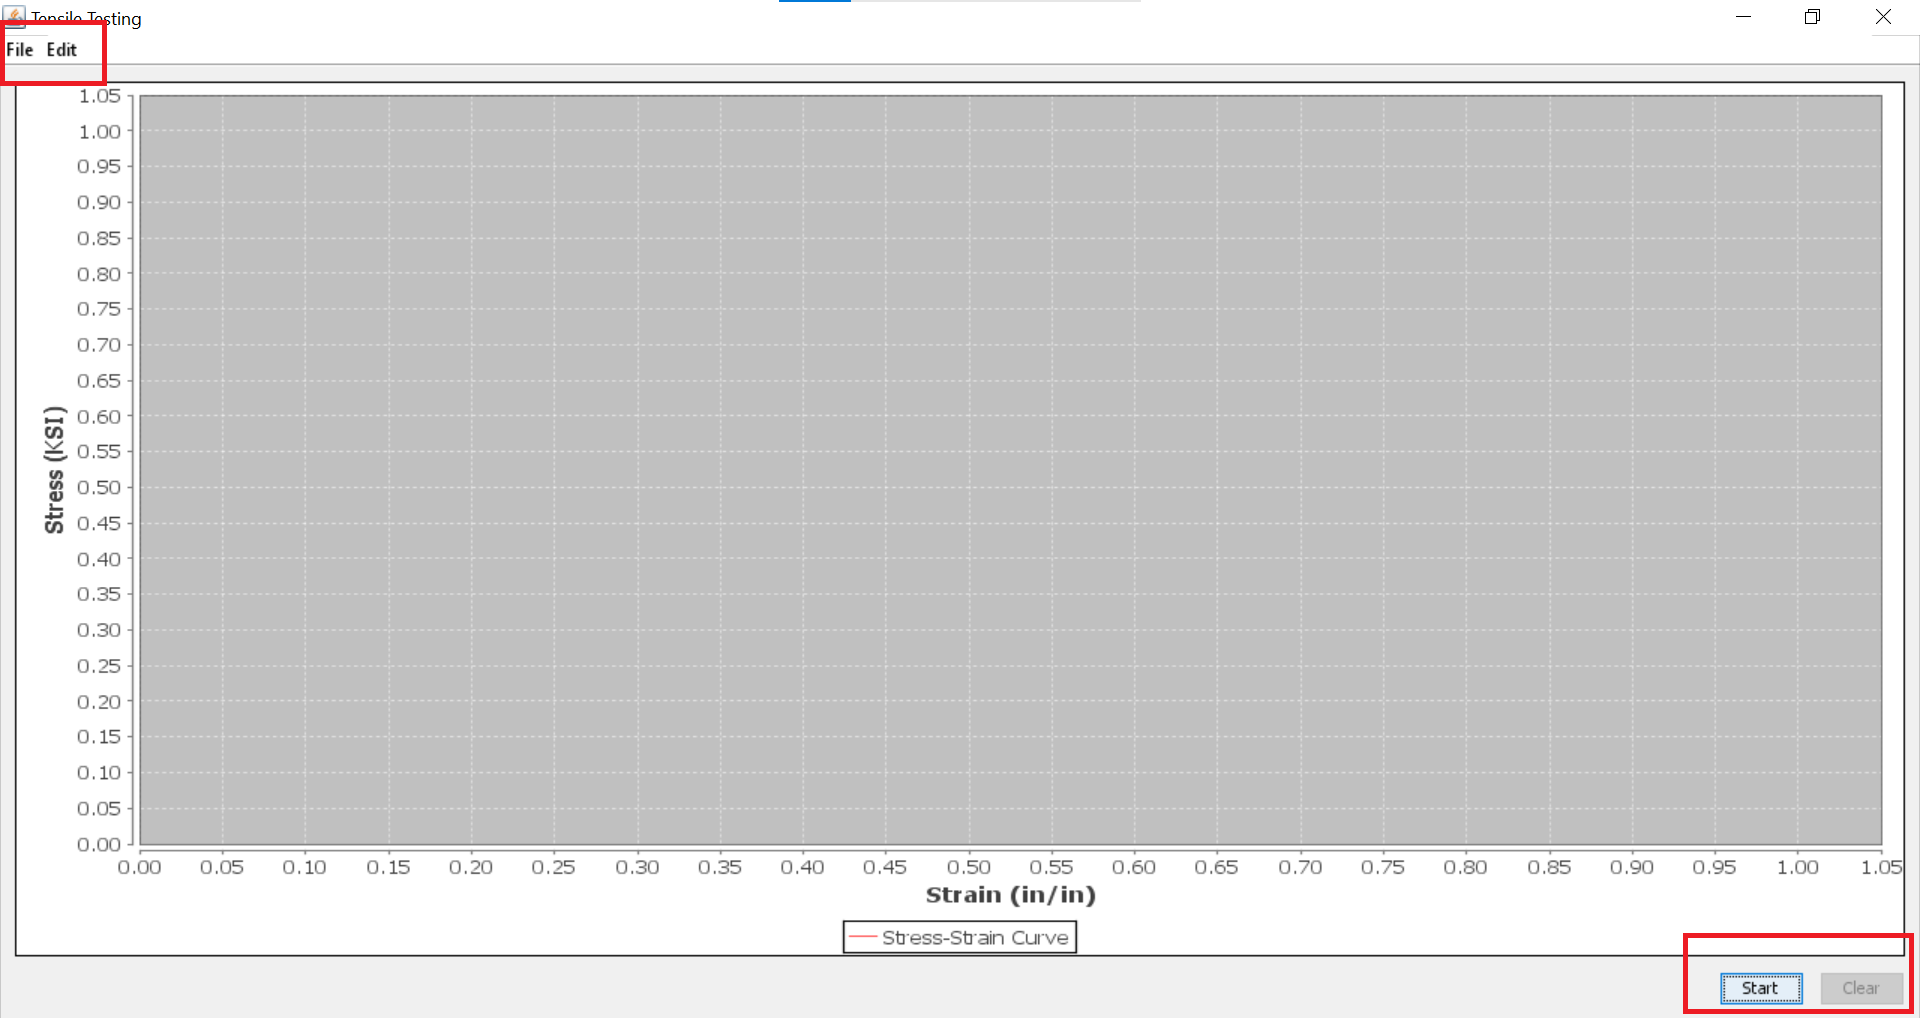
\includegraphics[scale=.45]{mainWindow}}
    \caption{Main Window}
\end{figure}

\subsection{Settings} \label{settingsSection}
Default settings can be changed by clicking on the ``File'' menu and then the ``Settings'' item or through the associated hotkey (see Table \ref{hotkeys}). Upon opening, the user will see options for force and elongation machine settings, and default gauge length and unit system.

\begin{figure}[H]
    \centering
    \frame{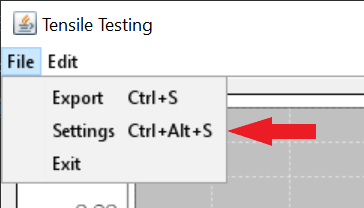
\includegraphics[scale=.75]{settingsItem}}
    \hspace{1em}
    \frame{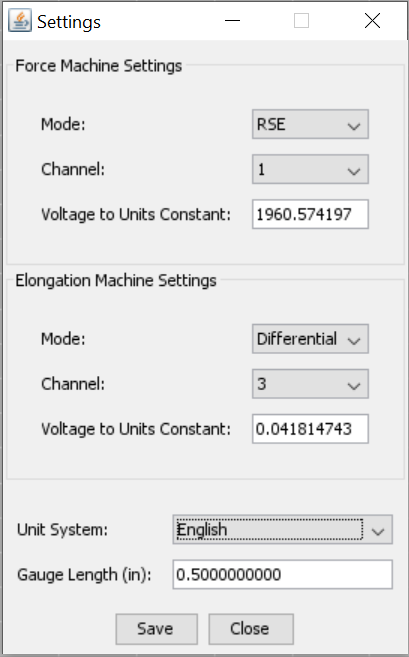
\includegraphics[scale=.75]{settingsWindow}}
    \caption{Settings Window}
\end{figure}
The ``Force Machine Settings'' and ``Elongation Machine Settings'' sections house all the information about the force machine and elongation machine currently connected. The appropriate channel and mode options must be selected for each machine as well as a calculated constant for converting voltage to real units. Note that for the ``RSE'' mode the channel options are 0-7, but for the ``Differential'' mode the options are only channels 0-4. This difference is because the ``RSE'' mode uses one channel and the ground channel, while the ``Differential'' mode uses two channels. Thus, if channel 0 is selected with Differential mode, the corresponding appropriate channels to use in the National Instruments device would be channels 0 and 1. Likewise, if channel 1 is selected with Differential mode, the channels to use would be channels 2 and 3. See Table \ref{settingsTable} for the default settings configuration for the machines used at time of release.

Refer to the diagram below for information about wiring.
\begin{figure}[H]
    \centering
    \frame{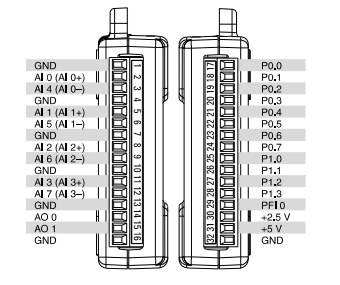
\includegraphics[scale=.75]{wiringDiagram}}
    \caption{Wiring Diagram}
\end{figure}

Once all values have been updated as desired, select the ``Save'' button to apply the changes. Exiting the window or choosing ``Cancel'' at any time will erase all unsaved changes to the settings. 
Note that in most cases, the user will not want to change these values since changes to these settings affect all other users as well and will be saved after the program is closed.
The user should be sure that what is changed is actually correct before continuing.

\subsection{Input Measurements} \label{inputSection}
Settings and measurements to be used for a specific test run can be updated and input by clicking the ``Input'' button, by selecting the ``Edit'' menu and then the ``Input Measurements'' item, or through the associated hotkey (see Table \ref{hotkeys}). 
\begin{figure}[H]
    \centering
    \frame{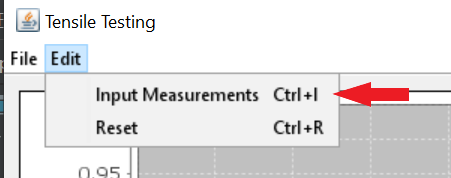
\includegraphics[scale=.5]{inputItem.png}}
    \hspace{1em}
    \frame{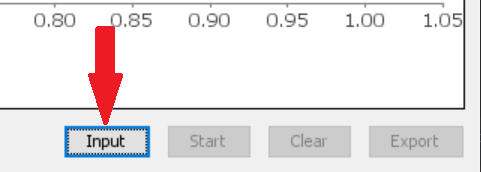
\includegraphics[scale=.75]{inputButton.png}}
    \caption{Inputting Measurements}
\end{figure}
Upon opening the input window, the unit system, gauge length, and cross-section measurements can be input accordingly. To prepare a test to run, select the desired unit system and double check that the gauge length value is correct. Note that it is unlikely that the gauge length value will be incorrect and the user should be sure that they actually wish to change this value. Next, choose the appropriate cross-section type for the current test sample (``Rectangular'' or ``Circular''). An input field for the corresponding type of measurement will appear, and the user can then input the appropriate value(s) measured from the specimen. After all values in the input window have been updated, select ``OK'' to save the values. If ``Cancel'' is selected or the window is closed at any time, no changes to the values will be saved. 
Note that these values will not be saved upon exiting the application and will not affect anything outside of the current instance of the application.
\begin{figure}[H]
    \centering
    \frame{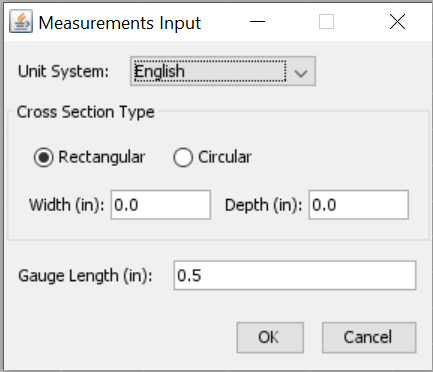
\includegraphics{inputWindow.png}}
    \hspace{1em}
    \frame{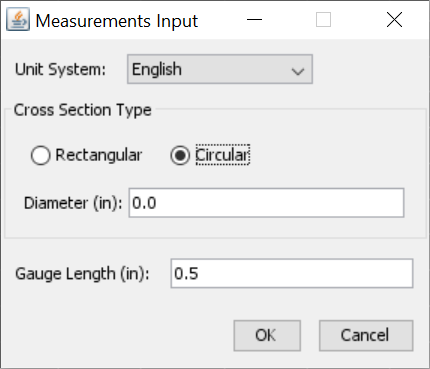
\includegraphics{inputWindowCircular.png}}
    \caption{Input Window}
\end{figure}

\subsection{Running a Test} \label{testSection}
Once the settings and input have been configured as desired and the specimen has been loaded into the machine with the extensometer, data collection can begin by selecting the ``Start'' button. Note that once data collection has started, this button will change to say ``Stop.'' Data collection can be terminated at the appropriate time by selecting the ``Stop'' button. Note that once the specimen has broken, the readings will become wildly scattered and completely wrong. \textbf{Thus, it is important that the user stops data collection as soon after the specimen has broken as possible to avoid this issue.}
\begin{figure}[H]
    \centering
    \frame{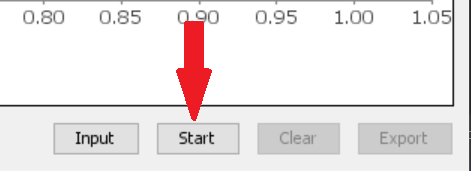
\includegraphics[scale=.75]{startButton.png}}
    \hspace{1em}
    \frame{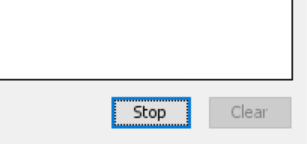
\includegraphics[scale=.75]{stopButton.png}}
    \caption{Start and Stop Data Collection}
\end{figure}
If the user wishes to change unit systems after data has been collected, this change can be accomplished by simply reopening the input window and selecting the desired unit system. Note that while the input values in the input window will not appear to change, they will be converted to the proper unit system in the exported file. \label{reset}After data collection has stopped, the ``Clear'' button will be enabled. Selection of this button will clear all data from the graph but will keep all input values the same. Note that the ``Reset'' item under the ``Edit'' menu can be used to both clear the data and restore all input values back to their default values. 
\begin{figure}[H]
    \centering
    \frame{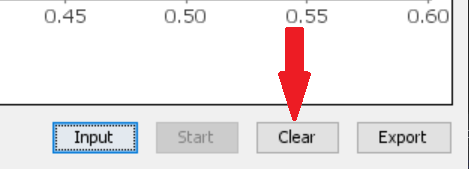
\includegraphics[scale=.75]{clearButton.png}}
    \hspace{1em}
    \frame{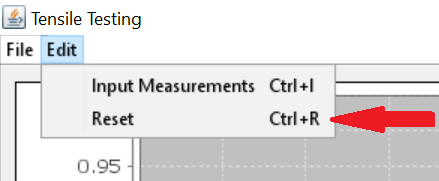
\includegraphics[scale=.75]{resetItem.png}}
    \caption{Clear and Reset}
\end{figure}

\subsection{Exporting Data} \label{exportSection}
Data can be exported by clicking the ``Export'' button, by selecting the ``Export'' item under the ``File'' menu, or through the associated hotkey (see Table \ref{hotkeys}).
\begin{figure}[H]
    \centering
    \frame{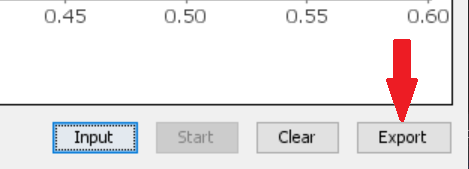
\includegraphics[scale=.75]{exportButton.png}}
    \hspace{1em}
    \frame{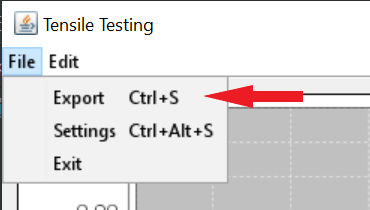
\includegraphics[scale = .55]{exportItem}}
    \caption{Exporting Data}
\end{figure}
When the export window appears, the user has the option to include the values they had previously input to calculate the stress-strain data along with the data itself in the export file. By default, this box will appear checked; uncheck the box to exclude this information from the saved file. Once the user has selected the desired options, click ``Export'' to choose the location and name of the saved file. Note that CSV files are opened in Excel by default on Windows machines. Also note that on the Otterbein University machines, data is erased when a user logs out of their account. Thus, it is necessary to store files somewhere other than the desktop itself or they will be deleted upon signing out. Also, if any graphs or calculations are done in Excel with the CSV file, they must be saved separately, as CSV files only include values and thus all other data will be lost. The user can change the file type to .xlsx to save it as an excel formatted file that will include any graphs or calculations.
\begin{figure}[H]
    \centering
    \frame{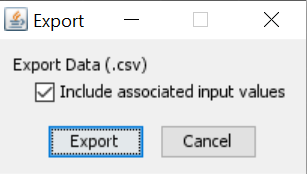
\includegraphics{exportWindow}}
    \caption{Export Window }
\end{figure}

\section{Calibration} \label{calibrationSection}
To convert voltage to units, an appropriate voltage constant is necessary. A tool is included to aid users in finding their own voltage to units constant. First, a user will need a means for retrieving data from the machine being tested. This process should include stopping for one second while the data is being collected from the National Instruments Device. After the technique is devised, the user should steadily increase the values, stopping at increments of the user's choosing (NOTE: adding more increments could possibly make the data more accurate). 

When the user ends at an increment, they should enter the ``add'' command to add the value to the dataset. Once complete, type the ``finished'' command and the tool will calculate a linear regression on the dataset. The resultant voltage to units constant will be displayed in the terminal. This value can then be entered into the appropriate field in the settings window to update the main software.

\section{Outside Resource Information} \label{resourceSection}

\subsection{Hardware}
This software is designed to work best with National Instruments USB-6009 device. It requires drivers to interface with the hardware found here:
\url{https://www.ni.com/en-us/support/downloads/drivers/download.ni-daqmx.html}

These drivers interface with the hardware and our software and are necessary to have the software work properly. If the drivers are not installed or are not recognizing the chip the software will not work properly. In addition, the National Instruments USB-6009 manual can be found here (\url{https://www.ni.com/pdf/manuals/371303n.pdf}) for more information on the chip itself. 

This software has been designed and tested on the Spec Tester from Accutek as well as an Epsilon Technology Core Extensometer. As such the default calibration are set to those machines. The software can use other machines in theory, but has not been tested on other machines. To use this software with other machines, the user must wire an amplified signal (giving a range between + or - 10 Volts) into a channel on the National Instruments chip. In addition, a linear regression test should be conducted on the voltage values vs the actual values read giving you volts to unit. In the settings, the voltage to units can be set as well as the channel and mode. The machine should specify what type of signal it gives and the manual for the National Instruments chip shows what configuration should be used.  

\subsection{Software}
This software requires that the Java Virtual Machine along with Java 8 be installed on the machine it is to be used on. This application is only meant to run for Windows and functionality/appearance is not guaranteed.

\pagebreak
\section{Appendix}

\begin{table}[H]
    \centering
    \rowcolors{2}{lightcyan}{bubbles}
    \begin{tabular}{|c|c|}
        \hline
        \rowcolor{columbiablue}
        Menu & Hotkey \\
        \hline
        File & Alt+F \\
        \hline
         Edit & Alt+E \\
         \hline
         Export & Ctrl+S \\
         \hline
         Settings & Ctrl+Alt+S \\
         \hline
         Exit & Alt+X \\
         \hline
         Input Measurements & Ctrl+I \\
         \hline
         Reset & Ctrl+R \\
         \hline
         
    \end{tabular}
    \caption{Hotkeys}
    \label{hotkeys}
\end{table}

\begin{table}[H]
    \centering
    \rowcolors{2}{lightcyan}{bubbles}
    \begin{tabular}{|c|c|}
        \hline
        \rowcolor{columbiablue}
        Option & Value\\
        \hline
        Force Mode & Differential \\
        \hline
        Force Channel & 3 \\
        \hline 
        Force Constant & 1960.574197 \\
        \hline 
        Elongation Mode & RSE \\
        \hline
        Elongation Channel & 1\\
        \hline
        Elongation Constant & 0.041814743\\
        \hline
        Unit System & English\\
        \hline
        Gauge Length & 0.5\\
        \hline
    \end{tabular}
    \caption{Default Settings for Machines}
    \label{settingsTable}
\end{table}

\subsection{Frequently Asked Questions}
\begin{enumerate}
    \item How do I update my channel and mode options?\\ 
    Default settings can be updated in the settings window (see \ref{settingsSection})
    \item What is the difference between the gauge length and unit system in the settings window versus the input window?\\
    The gauge length and unit system selected in the settings window will be saved and used as the preferred defaults in future uses of the application, while the input window values are what are actually used in calculations for a specific test. \textbf{It is unlikely that the settings will need to be changed unless a different extensometer is being used. Instead, change the values in the input window only.}
    \item How do I input the measurements of the specimen?\\
    Measurements can be input in the input window (see \ref{inputSection})
    \item I am using a cylindrical specimen, what measurements do I input?\\
    To use a cylindrical specimen, choose the ``Circular'' option in the input window (see \ref{inputSection})
    \item I collected data in one unit system but would like to view it in another? \\
    Unit systems can be changed in input window, even after data collection (see \ref{inputSection})
    \item How do I export my data?\\
    Data can be exported through the export window (see \ref{exportSection})
    \item How do I open my exported data file?\\
    Navigate to the location where the file was saved and double click; the file will automatically open in excel 
    \item How do I reset the application to run another test? \\
    Data can be cleared or the entire program can be reset through either the ``Clear'' button or the ``Reset'' item, respectively (see \ref{reset})
\end{enumerate}
\end{document}